
\section{Deferred Tessellation}


\label{sec:tessellation}

Tessellation is performed on each intersecting triangle. This stage is referred as deferred tessellation, because the tessellation happens after all of the intersections between triangles are computed, instead of clipping triangles incrementally at each intersection.

Many methods use CDT to perform tessellation on triangles. They treated triangle faces as convex triangulation zones, and intersections as constraints. However, CDT algorithms \cite{chew1989constrained,preparata2012computational} are performed in 2D. Even after mapping to three dimensions, implementing a plane-based CDT requires introduction of new planes. These new planes are used to guarantee that each subface is a triangle (see Fig. \ref{fig:iisect}d). We find double-precision is not enough to store the coefficients of these planes. Therefore, we choose not to add any new edges, performing minimal tessellation on each triangle. In this way, the subdivided faces are no more triangles, but general polygons.

\begin{figure}[t]
\centering
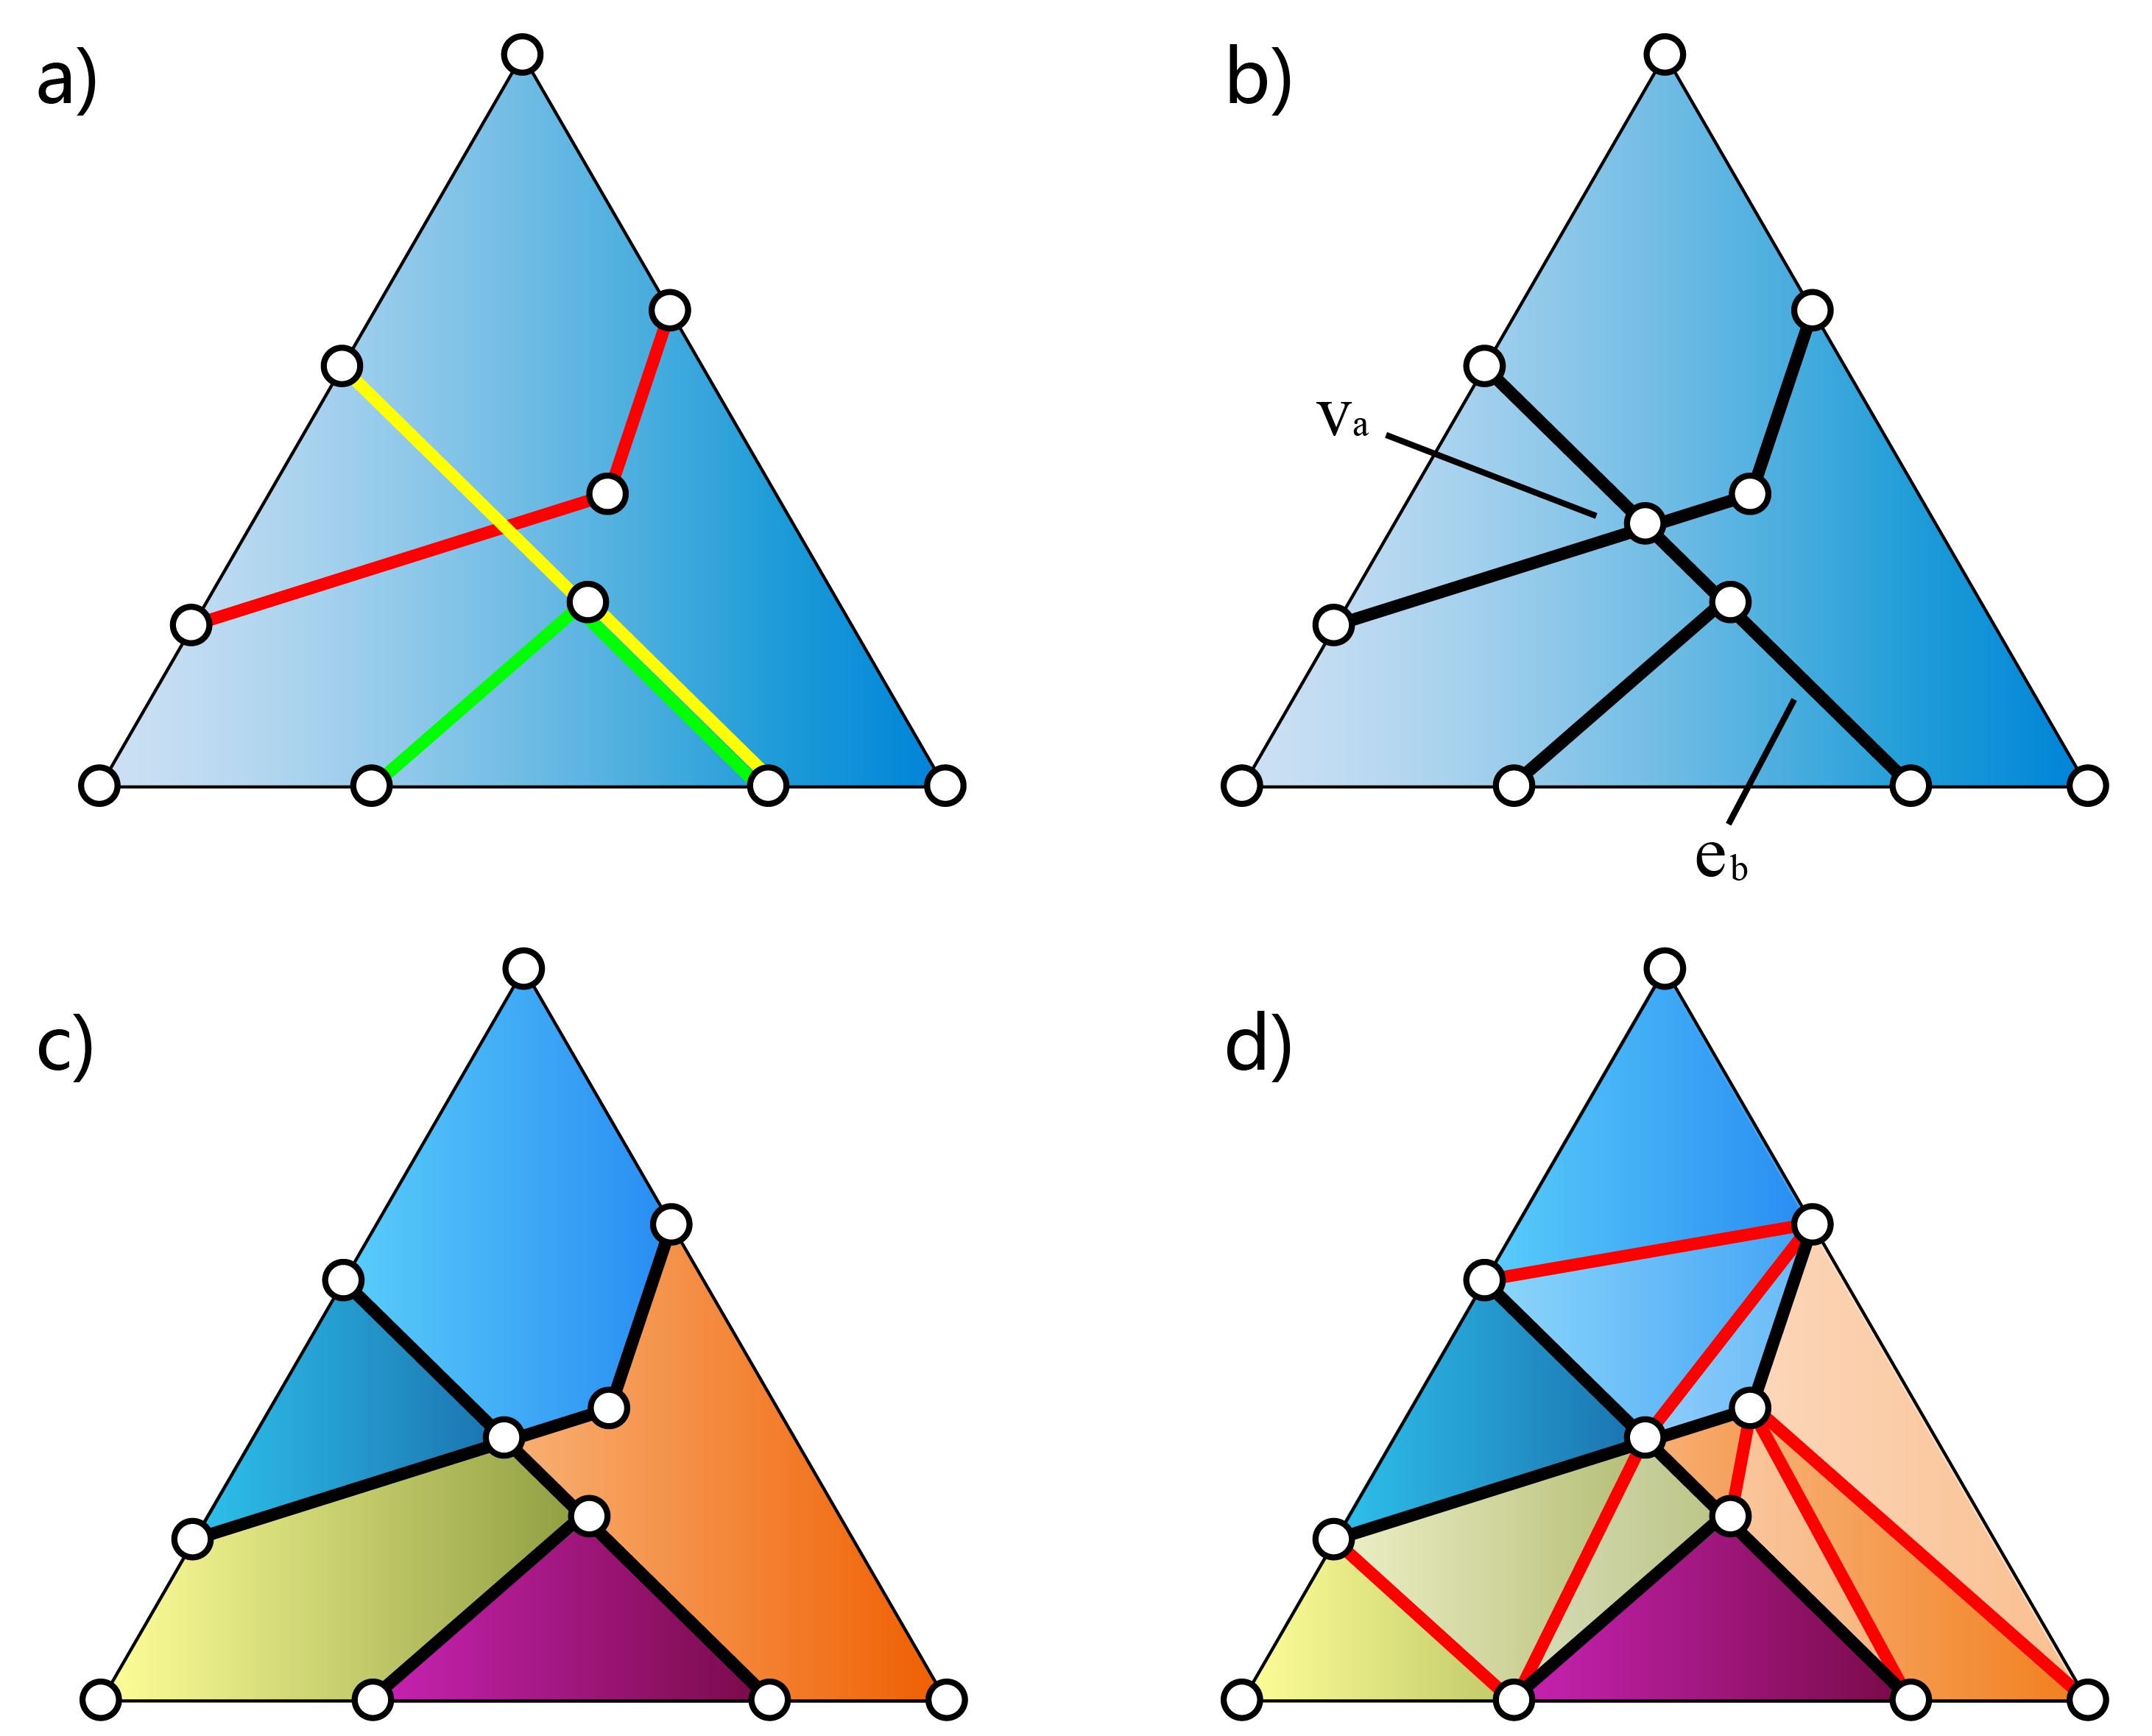
\includegraphics[width=3.5in]{boolean-04}
\caption{a) Different colors indicate that the intersections originate from different meshes. The yellow and red intersections intersect at a point. The yellow intersection overlaps with the green intersection. b) After refinement, we introduce a new vertex $\bm{v}_a$, and merge overlapping intersections into a single edge $\bm{e}_b$. c) Our tessellation method does not guarantee that all of the faces are triangular. d) If triangulation is performed, new edges (red lines) are introduced and double-precision is not enough to hold the plane coefficients of their P-reps.}
\label{fig:iisect}
\end{figure}


In our method we first perform intersection refinement to ensure that intersections intersect each other only on end points. After that, we perform our minimal tessellation based on \emph{tess-graph}, a graph-like description of the intersections on a given face.

\subsection{Intersection Refinement}

\label{sec:refine}

Intersection vertices can be introduced by the intersection of three triangles, in addition to intersections between an edge and a triangle. Triangle-triangle intersection tests only compute the latter. Thus, it is necessary to refine these triangle-triangle intersections before the final tessellation.

Intersection refinement is performed on the scope of each intersecting triangle. For triangle face $t$, we collect all of the intersections on $t$ as a set $\bm{\Gamma}(t)$ and refine them together. We also include the three edges of $t$ in $\bm{\Gamma}(t)$, because the edges are also involved in the step of subfaces extraction. In $\bm{\Gamma}(t)$, the three edges are represented by PBI-reps. The neighboring faces $\mathcal{N}$ are set as $N/A$ because they do not have a neighboring face. Other PBI-rep components can be determined by the P-reps of the edges. The refinement of $\bm{\Gamma}(t)$ is done using only plane-based geometric predicates, in the following three steps.


\vspace{0.5em}
\noindent \textbf{Coincidence elimination}~~~~
We merge coincidence intersections that have the same end points. Intersections are undirected, so intersections with inverse end points are also coincident. The PBI-rep of the merged intersection is inherited from either of the original intersections, except for the neighboring faces $\mathcal{N}$. The neighboring faces of the merge intersection is the union of all the neighboring faces of original ones. It means from now on, an intersection may have neighboring faces from different primitives.

\vspace{0.5em}
%Intersection refinement is performed locally
\begin{wrapfigure}{r}[0in]{0in}
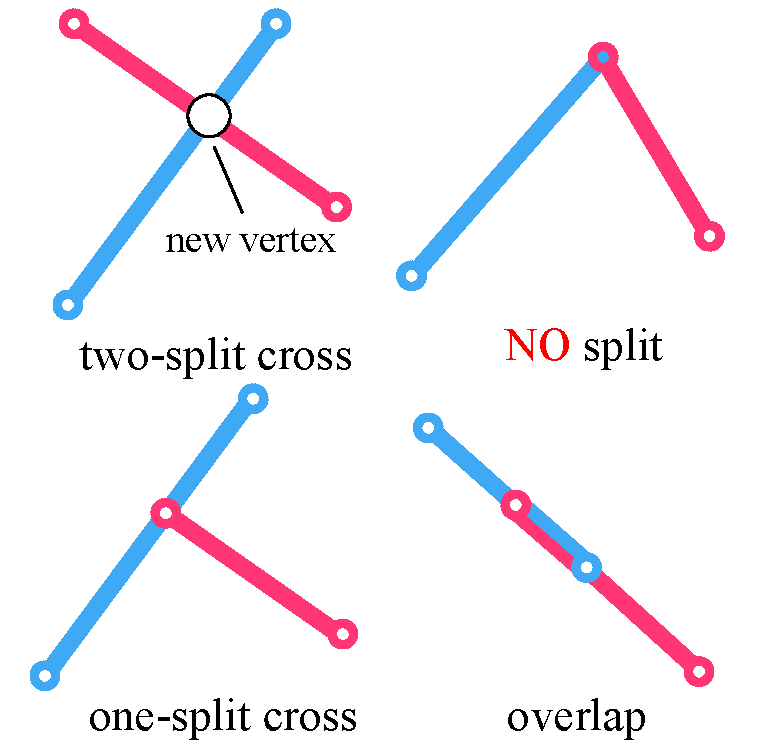
\includegraphics[width=1.5 in]{resolve}
%\caption{Plane-based representation of triangle}
\end{wrapfigure}
\noindent\textbf{Intersection resolving}~~~~
Each pair of intersections is tested if they intersect in any location other than end points. The tested intersections should be from different primitives, since primitive inputs are free of self-intersecting. The three conditions of intersections are illustrated on the right. When two intersections intersect, at least one of them is split. New vertices may be introduced, whose P-reps are intersections between the common plane and the two $\bm{P}_{ext}$ of the PBI-reps of the two intersections. Because one intersection may be in contact with more than one other intersection, this splitting is deferred until all of the splitting points are found. The PBI-reps of the split segments inherit that of their father's, except for $\bm{P}_0, \bm{P}_1$, since the split segments have different end points.

\vspace{0.5em}
\noindent \textbf{Coincidence elimination (revisited)}~~~~
If two intersections are collinear, resolving their overlap may produce new coincident intersections. Therefore, the first step of the process is repeated here.

\subsection{Tessellation by Tess-Graph}
\label{sec:tess}

To perform tessellation and extract subfaces, we use tess-graph, which is the graph description of the tessellated face topology. For each intersecting triangle face, we construct a tess-graph according to the refined set of intersections. Nodes of the tess-graph represent the end points of intersections, and connections between nodes represent intersections. The construction of a tess-graph is straightforward, and readers should be able to determine the details.


After the tess-graph is constructed, we extract subfaces by   valid loops. A valid loop is a loop in tess-graph which satisfy two criteria: 1) the direction of the loop should correspond with the face normal, and 2) consecutive connections on the loop should be adjacent by circular order. Each valid loop corresponds to an intersection-free face. After all of the valid loops are determined from the tess-graph, the corresponding face is tessellated (see Fig. \ref{fig:cadj}). To facilitate face classification, we also store neighboring faces in the edges of the new faces. Because the edges have one-to-one correspondence to the connections in tess-graph , and the connections have one-to-one correspondence to the PBI-reps, the neighboring faces of edges is determined from the corresponding PBI-reps.

\begin{figure}[t]
\centering
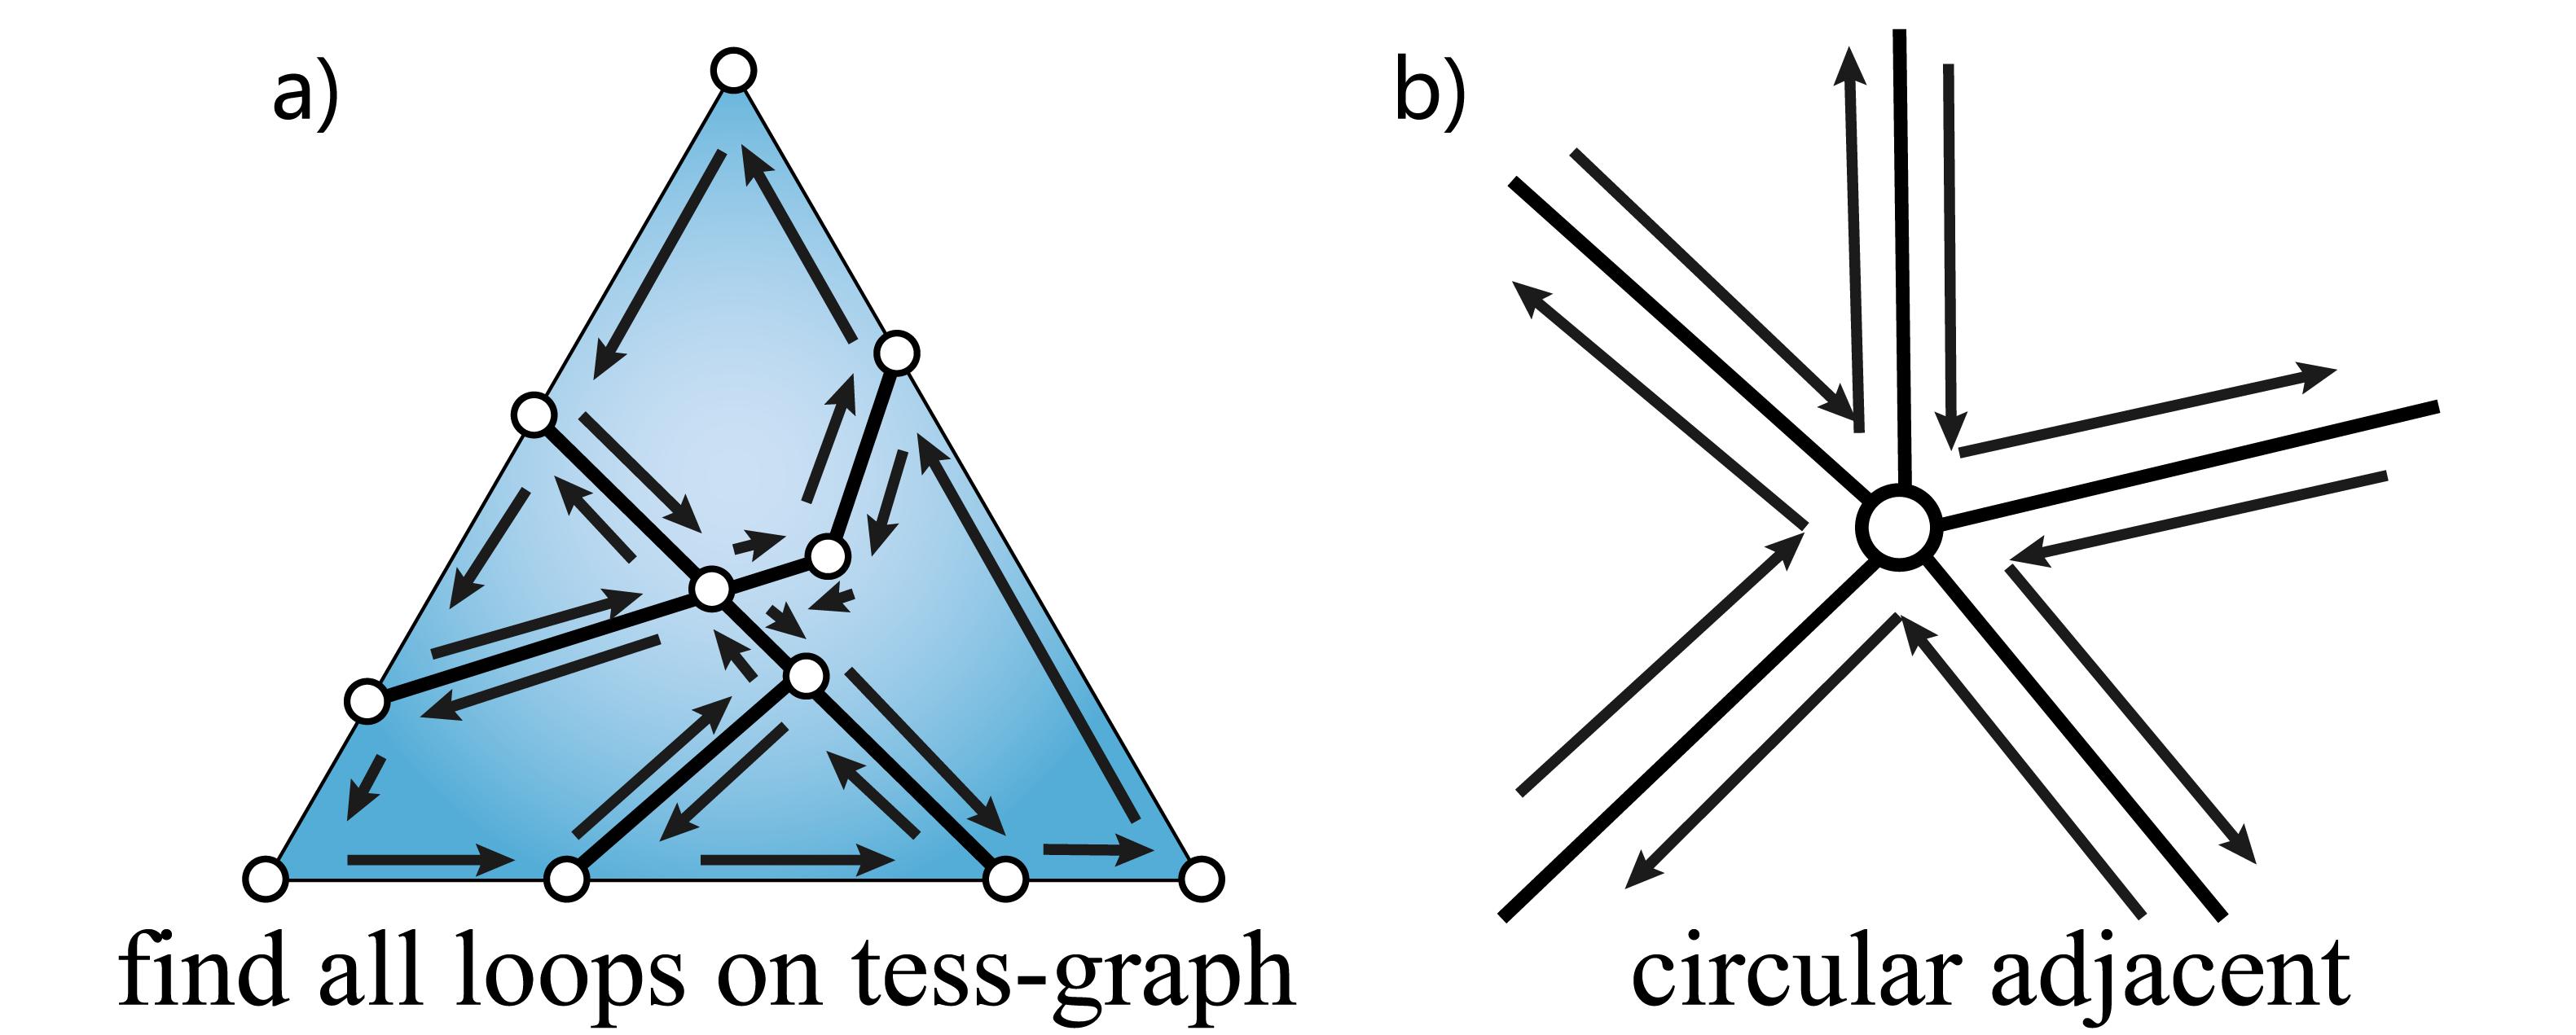
\includegraphics[width=3in]{boolean-05}
\caption{a) To tessellate a triangle, we find all of the valid loops on a tess-graph. The direction of the loops must be coherent with the triangle normal (assuming here that the normal points to the outside of the paper). b) Each circular adjacent edge pair is an angle of the tessellated polygon.}
\label{fig:cadj}
\end{figure}
